\documentclass[twoside]{article}

\usepackage{graphicx}
\usepackage{float}
\usepackage[math]{kurier}
\usepackage[sc]{mathpazo}
\usepackage[ruled]{algorithm2e}
\usepackage{enumitem}

\renewcommand{\sfdefault}{kurier}

\usepackage{graphics}
\setlength{\oddsidemargin}{0.25 in}
\setlength{\evensidemargin}{-0.25 in}
\setlength{\topmargin}{-0.6 in}
\setlength{\textwidth}{6.5 in}
\setlength{\textheight}{8.5 in}
\setlength{\headsep}{0.75 in}
\setlength{\parindent}{0 in}
\setlength{\parskip}{0.1 in}

\newcounter{lecnum}
\renewcommand{\thepage}{\thelecnum-\arabic{page}}
\renewcommand{\thesection}{\thelecnum.\arabic{section}}
\renewcommand{\theequation}{\thelecnum.\arabic{equation}}
\renewcommand{\thefigure}{\thelecnum.\arabic{figure}}
\renewcommand{\thetable}{\thelecnum.\arabic{table}}


\newcommand{\lecture}[3]{
   \pagestyle{myheadings}
   \thispagestyle{plain}
   \newpage
   \setcounter{lecnum}{#1}
   \setcounter{page}{1}
   \noindent
   \begin{center}
   \framebox{
      \vbox{\vspace{2mm}
    \hbox to 6.28in { {\bf \sffamily AA 274: Principles of Robotic Autonomy
                        \hfill Winter 2019} }
       \vspace{4mm}
       \hbox to 6.28in { {\sffamily{\Large \hfill Lecture #1: #2  \hfill}} }
       \vspace{2mm}
      \vspace{2mm}}
   }
   \end{center}
   \markboth{Lecture #1: #2}{Lecture #1: #2}

   \vspace*{4mm}
}



%%%%%%%%%%%%%%%%%%%%%%%%%%
%document
\begin{document}
\lecture{14}{SLAM II: graph-based SLAM and particle-filter SLAM}{}

\section{Introduction}

During the last lecture, we covered an important class of SLAM algorithms based on EKF. However, one main issue with EKF-SLAM is that it tends to scale quite poorly with the number of features. Furthermore, this method relies on a linearization process performed globally, which is only efficient when the estimate is close to the truth.
In this lecture, we cover two additional algorithms for SLAM that  don't suffer from these limitations: graph-based SLAM and particle-filter SLAM. We give a very quick overview of graph SLAM before moving on to particle-filter SLAM, often referred to in literature as Fast-SLAM. This will give us a good overview of the different techniques used in localization.

\section{Graph SLAM}

While EKF's goal was to solve the SLAM problem online, the Graph SLAM algorithm aims at solving the full-scale SLAM problem.  More precisely, we want to get an estimate of the map $m$  and of the entire robot's path -- i.e. the whole state history $x_{1:t}$ and not just an estimate of the state $x_t$ at time $t$ --  conditioned on the measurement and control history:
\begin{equation}
p(x_{1:t}, m, c_t | z_{1:t}, u_{1:t}) \nonumber
\end{equation}
In full generality, we also want to get an estimate of the correspondence variable $c_t$ that allows us to correlate a measurement with the features. We are not interested in $c_t$ \textit{per se}, but it is necessary in order to estimate the map and the state history.

In Graph SLAM, we interpret the SLAM problem as a graph optimization problem. We associate nodes of the graph with robot locations and feature locations, and we connect these nodes with constraints. The constraints between two robot locations have to obey the motion model, while the constraints between a robot location and a map feature obey the observation model.

\begin{figure}[H]
\centering
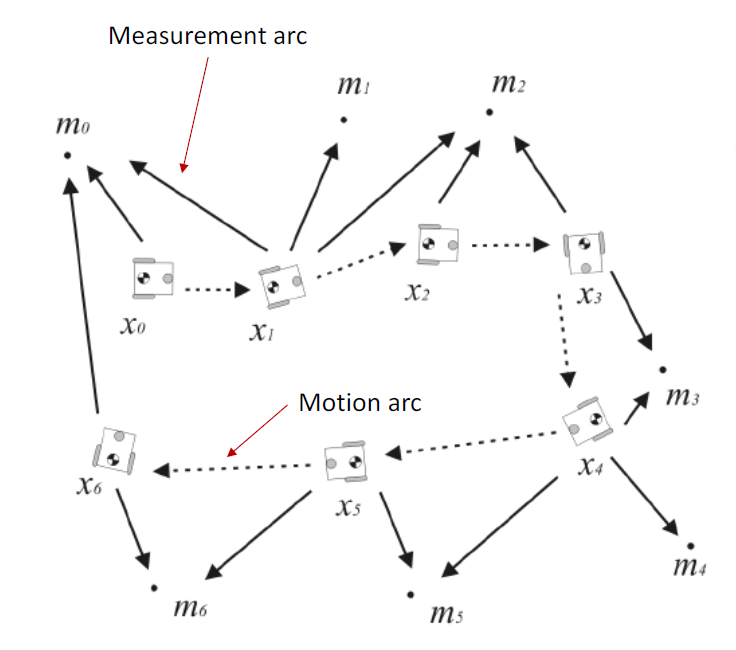
\includegraphics[scale=0.4]{graphSLAM_fig1}
\caption{Graph representation of a simple SLAM problem.}
\end{figure}

In Figure 14.1 above,  the robot moves from $x_0$ to $x_6$ while observing a set of features $m_0$ to $m_6$. As stated above, the nodes of the graph are the robot positions and the features. The edges can be either motion arcs representing relative distance between two consecutive robot poses subject to the motion model, or measurement arcs representing the distance to a feature, conditioned on the robot pose and subject to the measurement model.

The key idea is to interpret these edges -- or constraints -- as \textit{soft probabilistic constraints}, that we can represent as springs (see Figure 14.2 below). The intuition is that a spring constant represents the uncertainty for a certain measurement model, i.e. the difference between the expected measurement and the actual measurement. The approach of the algorithm is then to find the best estimate of the robot poses and feature locations as the state of minimal energy for that spring network. In other words, the most probable joint estimate of robot poses and feature locations minimizes the energy of the network. Note that we usually linearize the constraints and represent them as quadratic constraints.

\begin{figure}[H]
\centering
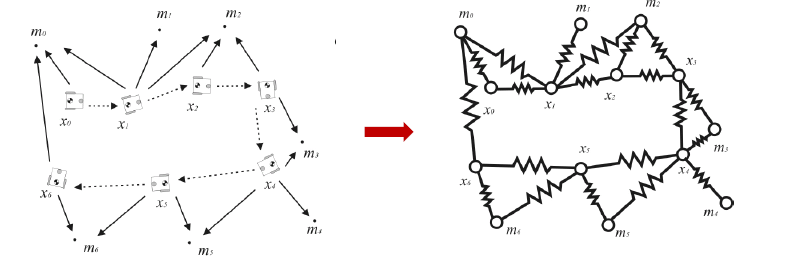
\includegraphics[]{graphSLAM_fig2}
\caption{Interpretation of the SLAM graph as a springs network. The optimal estimate is obtained by minimizing the energy of the network.}
\end{figure}

An advantage of Graph SLAM is that we can solve the global problem directly in batch, which gives us a more robust estimate. However, Graph SLAM requires to solve a non-linear least-square optimization problem, which can be a lot more complex to solve than EKF or Particle-filter SLAM, as we will see.

You can find more information on the Graph SLAM algorithm in chapter 11 of [2].

\section{Particle Filter SLAM}

The last class of SLAM algorithms we will focus on is Fast-SLAM. This is a powerful algorithm that has been used successfully in a variety of applications and  it is a natural continuation of what we've seen thus far in particle filtering.

The idea here is to approximate our belief with a set of particles. The difference with particle localization is that we want to simultaneously estimate the robot pose as well as the map:
\begin{equation}
p(x_{1:t}, m, c_t | z_{1:t}, u_{1:t}) \nonumber
\end{equation}If we apply particle filtering to SLAM in a naive way, however, we will be confronted to the curse of dimensionality, as the number of particles will grow too large for any practical implementation. More precisely, it can be shown that the number of particles will grow exponentially with the number of dimensions.

The key insight of Particle Filtering SLAM is that knowing the true robot's path makes features conditionally independent. As we will prove, one can then factor the SLAM posterior $p(y_{1:t}|z_{1:t},u_{1:t},c_{1:t})$ into the product of the posterior over the path,  $p(x_{1:t}|z_{1:t},u_{1:t},c_{1:t})$ , and the posteriors over each of the $N$ map features, $p(m_n|x_{1:t},z_{1:t},c_{1:t})$ :

\begin{equation}
p(y_{1:t}|z_{1:t},u_{1:t},c_{1:t}) = p(x_{1:t}|z_{1:t},u_{1:t},c_{1:t})\prod_{n=1}^Np(m_n|x_{1:t},z_{1:t},c_{1:t})\nonumber
\end{equation}
The intuition behind the conditional independence of features given the true path is made clearer in the context of a dynamic Bayesian network:

\begin{figure}[H]
\centering
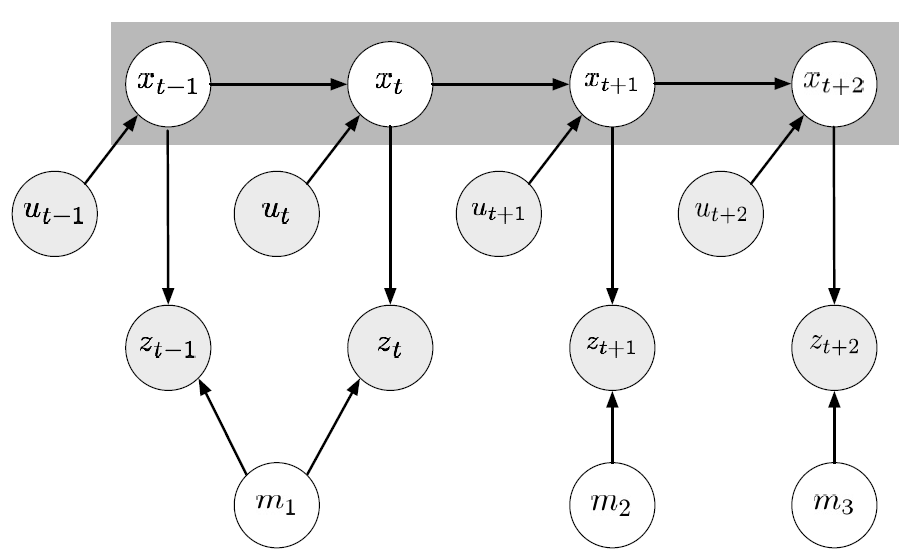
\includegraphics[scale=0.5]{fastSLAM_fig1}
\caption{Interpretation of SLAM as a Bayesian network problem.}
\end{figure}


Each measurement $z_t$ is a function of the state $x_t$ (the robot pose), and -- obviously -- of the feature $m_n$ that this measurement corresponds to. Note that for simplicity, we will restrict our analysis to the case where we only measure \textit{one} feature $m_n$ at a time. One can relax this assumption in the case of batch measurements by treating each measurement $z_{t,m}$ sequentially, assuming that the position $x_t$ of the robot is kept constant.

We see form Figure 14.3 above that, given the position $x_t$, the measurement $z_t$ is independent from the rest of the path and therefore the estimations of each feature location become independent problems.

\subsection{Posterior Factorization}
As mentioned above, we would like to express the following SLAM posterior $p(y_{1:t}|z_{1:t},u_{1:t},c_{1:t})$ as

\begin{equation}
p(y_{1:t}|z_{1:t},u_{1:t},c_{1:t}) = p(x_{1:t}|z_{1:t},u_{1:t},c_{1:t})\prod_{n=1}^Np(m_n|x_{1:t},z_{1:t},c_{1:t})\nonumber
\end{equation}
\\

\textbf{Step 1:}

To start, we apply Bayes' rule to the posterior and split it into the posterior for the path times the posterior for map features:
\begin{equation}
p(y_{1:t}|z_{1:t},u_{1:t},c_{1:t}) = p(x_{1:t}|z_{1:t},u_{1:t},c_{1:t})p(m|x_{1:t},z_{1:t},u_{1:t},c_{1:t})
\end{equation}

Since the feautures do not depend on the control history, we can drop the condition on $u_{1:t}$ in the posterior for the map features. Our equation for the SLAM posterior becomes:

\begin{equation}
p(y_{1:t}|z_{1:t},u_{1:t},c_{1:t}) = p(x_{1:t}|z_{1:t},u_{1:t},c_{1:t})p(m|x_{1:t},z_{1:t},c_{1:t})
\end{equation}

We are almost at our goal. Now we need to express $p(m|x_{1:t},z_{1:t},c_{1:t})$ as $\prod_{n=1}^Np(m_n|x_{1:t},z_{1:t},c_{1:t})\nonumber$

In order to do so, we will go through two more steps.
\\

\textbf{Step 2.a}

We have a total of $n$ features. We will first consider the case where the correspondence at time $t$ is not for feature $n$; i.e. $c_t \neq n$. In this case, the posterior of feature $m_n$ is not dependent on $c_t$ and we can write:

\begin{equation}
p(m_n|x_{1:t},z_{1:t},c_{1:t}) = p(m_n|x_{1:t},z_{1:t},c_{1:t-1})
\end{equation}
\\

\textbf{Step 2.b}

In the case where the correspondence at time $t$ is for feature $n$ ($c_t = n$), we can apply Bayes' rule:

\begin{equation}
p(m_{c_t}|x_{1:t},z_{1:t},c_{1:t}) = \frac{p(z_t|m_{c_t}, x_{1:t},z_{1:t-1},c_{1:t})p(m_{c_t}|x_{1:t},z_{1:t-1},c_{1:t})}{p(z_t|x_{1:t},z_{1:t-1},c_{1:t})}
\end{equation}
\\

\textbf{Step 3}

To factor $p(m|x_{1:t},z_{1:t},c_{1:t})$ into $\prod_{n=1}^Np(m_n|x_{1:t},z_{1:t},c_{1:t})\nonumber$, we will use a proof by induction.
\\

\underline{Induction Hypothesis:}

assume that, at $t-1$,
\begin{equation}
p(m|x_{1:t-1},z_{1:t-1},c_{1:t-1}) = \prod_{n=1}^Np(m_n|x_{1:t-1},z_{1:t-1},c_{1:t-1})\nonumber
\end{equation}
\\

\underline{Induction Step:}

at time $t$,
\begin{equation}
p(m|x_{1:t},z_{1:t},c_{1:t}) = \frac{p(z_t|m,x_{1:t},z_{1:t-1},c_{1:t})p(m|x_{1:t},z_{t-1}, c_{t})}{p(z_t|x_{1:t},z_{1:t-1},c_{1:t})}
= \frac{p(z_t|m,x_{1:t},c_{1:t})p(m|x_{1:t-1},z_{t-1}, c_{t-1})}{p(z_t|x_{1:t},z_{1:t-1},c_{1:t})}
\end{equation}

So far we just applied Bayes' rule and assumed the features are not dependent on measurements, nor are they dependent on the current state $x_t$ or the current correspondence $c_t$. We now can apply our induction hypothesis to obtain:

\begin{equation}
p(m|x_{1:t},z_{1:t},c_{1:t}) = \frac{p(z_t|m,x_{1:t},c_{1:t})}{p(z_t|x_{1:t},z_{1:t-1},c_{1:t})}\prod_{n=1}^Np(m_n|x_{1:t-1},z_{1:t-1},c_{1:t-1})\nonumber
\end{equation}

Among the $N$ features, there is one that is matched with the correspondence at time $t$.

\begin{equation}
p(m|x_{1:t},z_{1:t},c_{1:t}) = \frac{p(z_t|m,x_{1:t},c_{1:t})}{p(z_t|x_{1:t},z_{1:t-1},c_{1:t})} p(m_{c_t}|x_{1:t-1},z_{1:t-1},c_{1:t-1})\prod_{n\neq c_t}p(m_n|x_{1:t-1},z_{1:t-1},c_{1:t-1})\nonumber
\end{equation}

In Step 2.a, we found an expression for $p(m_n|x_{1:t-1},z_{1:t-1},c_{1:t-1})$ when $n \neq c_t$. In Step 2.b, we found an expression for $p(m_{c_t}|x_{1:t-1},z_{1:t-1},c_{1:t-1})$. Plugging those expression into equation (14.12) above and simplifying, we get:

\begin{equation}
p(m|x_{1:t},z_{1:t},c_{1:t}) = p(m_{c_t}|x_{1:t},z_{1:t},c_{1:t})\prod_{n=1}^Np(m_n|x_{1:t-1},z_{1:t-1},c_{1:t-1})\nonumber = \prod_{n=1}^Np(m_n|x_{1:t},z_{1:t},c_{1:t})\nonumber
\end{equation}

Thus, assuming our factorization holds for $t-1$, we proved that it holds for $t$. Through induction, we proved that the factorization $p(m|x_{1:t},z_{1:t},c_{1:t}) = \prod_{n=1}^Np(m_n|x_{1:t},z_{1:t},c_{1:t})\nonumber$ holds for all $t$.

Going back to the expression in Step 1, we can plug our induction results into (14.5) to obtain:

\begin{equation}
p(y_{1:t}|z_{1:t},u_{1:t},c_{1:t}) = p(x_{1:t}|z_{1:t},u_{1:t},c_{1:t})\prod_{n=1}^Np(m_n|x_{1:t},z_{1:t},c_{1:t})\nonumber
\end{equation}

\subsection{Proof by Induction, a General Guide}
This section is a more detailed guide on proof by induction. In general, when we want to use induction to prove a statement holds for all the elements of a sequence, we go through the following steps.

\underline{Base Case:}
We must check that our statement holds for the first value of the sequence. For example, if we want to prove that the sum of the first $N$ integers is $\frac{N(N+1)}{2}$, we must check that "the sum of the first 1 integers" (i.e. 1) is indeed equivalent to that expression.

\begin{equation}
\frac{1(1+1)}{2} = 1
\end{equation}

\underline{Induction Hypothesis:}
Assume the statement holds for some $k^{th}$ element in our sequence. For our example, assume the sum of the first $k$ integers is equal to $\frac{k(k+1)}{2}$ for some integer $k$.

\underline{Induction Step:} Use our induction step to prove that the statement holds for $(k+1)^{th}$ element in our sequence.

\begin{equation}
1 + 2 + 3 +... + k + (k+1) = \frac{k(k+1)}{2} + (k+1) = (k+1)(\frac{k}{2} + 1) = (k+1)(\frac{k+2}{2})
\end{equation}

We just proved the statement for the $(k+1)^{th}$ instance!

What does this mean? We showed that the statement is true for the first case (base case); we also showed that the statement being true for one case means it is true for the next (induction hypothesis and step). Thus, the statement is true for the second element of our sequence, which also means it holds for the third, and the fourth... It is therefore true for all elements of our sequence.



\section{Fast SLAM}
\subsection{With Known Correspondences}

Fast SLAM is a solution to the SLAM problem with unknown data association. The idea of Fast SLAM is to exploit the factorization of the posterior. This is particularly useful in how we keep track of filters. We treat each particle as a multi-dimensional vector. The first component $x_t^{[k]}$ corresponds a particle filter that shows our hypothesis about the robot pose. We then keep track of a set of EKF filters for each feature. Each filter is modeled as a Gaussian and thus, we keep track of a mean $\mu$ and a covariance $\Sigma$. Since there are $m$ particles and $n$ features, there are $m*n+1$ filters. We are able to do this two step approach as a result of the conditional independence of each feature. In this sense, Fast SLAM is a hybrid combination between particle filtering for the robot pose and EKF filtering with respect to each feature conditional on robot hypotheses with respect to each robot pose. Each filter keeps track of one specific feature.

\begin{equation}
Y_t^{[k]} = <x_t^{[k]} , \mu_{1,t}^{[k]} , \Sigma_{1,t}^{[k]} , ... ,\mu_{[N,t]}^{[k]} , \Sigma_{N,t}^{[k]} >\nonumber
\end{equation}

In order to keep track of the robot pose and all future locations, we must propagate forward a particle from time $t-1$ to $t$. This is done in the following three steps by incorporating a measurement $z_{t}$ and a knowledge of the control input $u_{t}$.

Steps:
\\
\hspace*{5mm}
1. Extend path posterior
\\
\hspace*{5mm}
2. Update the observed feature estimates
\\ \hspace*{5mm}
3. Resample

\textbf{Extend Path Posterior}

Forward propagation is done by using the motion model. Since we sample probabilistically, the hypothesis about the robot pose at time $t$ is related to the previous hypothesis about the robot pose and the control input. In this approach, $x_{t-1}^{k}$ is the k-th hypothesis about the robot pose at time $t-1$.

\begin{equation}
x_t^{k} \hspace*{1mm} \alpha \hspace*{1mm} p( x_t^{k} | x_{t-1}^{k} , u_t)\nonumber
\end{equation}

\textbf{Update the Observed Feature Estimates}

The updating of a feature estimate depends on whether that feature is observed at time $t$. The simplest case occurs when a feature is not observed. For this case, we keep our Gaussian estimate of the feature constant through the time step since we have no new information about the specific feature.

\begin{equation}
<\mu_{n,t}^{[k]},\Sigma_{n,t}^{[k]}> \hspace*{1mm} = \hspace*{1mm} <\mu_{n,t-1}^{[k]},\Sigma_{n,t-1}^{[k]}>\nonumber
\end{equation}

If we do observe a feature at time t, then that measurement will give us additional information that we can use to refine our estimate. The update is performed by exploiting Bayes' rule where the probability of the location of a feature given the history is equivalent to the probability of the measurement multiplied by the probability of the feature given the history up to the previous time step and a normalization factor $\eta$.

\begin{equation}
p(m_{c_t} | x_{1:t}, z_{1:t}, c_{1:t}) = \eta p(z_t | m_{c_t},x_t,c_t)p(m_{c_t} | x_{1:t-1}, z_{1:t-1}, c_{1:t-1})
\end{equation}

The measurements up to this point are Gaussian and we must linearize the model to ensure that the new estimate is as well.

\begin{equation}
h(m_{c_t},x_t^{[k]}) = h(\mu_{c_t,t-1}^{[k]},x_t^{[k]})+h^{'}(\mu_{c_t,t-1}^{[k]},x_t^{[k]})(m_{c_t}-\mu_{c_t,t-1}^{[k]})
\end{equation}

Once we linearize the measurement model, we must propagate forwards the mean and covariance through standard EKF update procedures.

\begin{equation}
K_t^{[k]} \hspace*{1mm} = \hspace*{1mm} \Sigma_{c_t,t-1}^{[k]}[H_t^{[k]}]^T(H_t^{[k]} \Sigma_{c_t,t-1}^{[k]}[H_t^{[k]}]^T+Q_t)^{-1}
\end{equation}

\begin{equation}
\mu_{c_t,t}^{[k]} \hspace*{1mm} = \hspace*{1mm} \mu_{c_t,t-1}^{[k]}+K_t^{[k]}(z_t-\hat{z}_t^{[k]})
\end{equation}

\begin{equation}
\Sigma_{c_t,t}^{[k]} \hspace*{1mm} = \hspace*{1mm} (I-K_t^{[k]}H_t^{[k]})\Sigma_{c_t,t-1}^{[k]}
\end{equation}

\textbf{Resample}

Because step 1 generates pose $x_{t}$ only in accordance with the most recent control $u_{t}$, paying no attention to the measurement $z_{t}$, we then need to resample the particles to correct for the inevitable mismatch.

\begin{figure}[H]
\centering
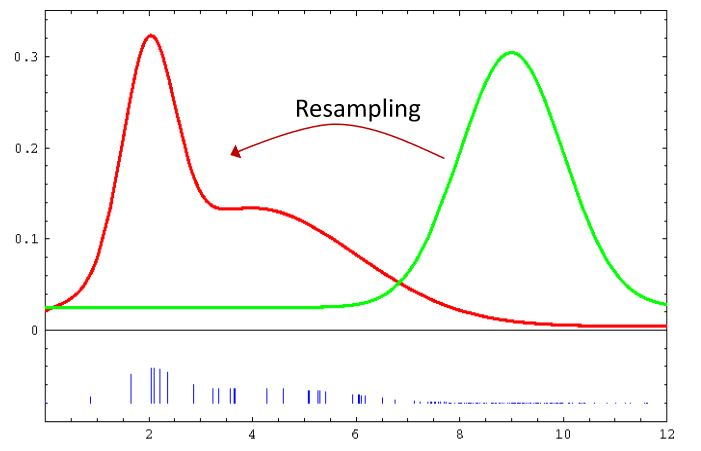
\includegraphics[scale=0.5]{Resampling_Figure}
\caption{Example of Resampling}
\end{figure}

When resampling the particles, it is important to first determine the weights of each hypothesis, based on which ones are most favorable.  At this stage, path particles are distributed according to the following probability function, which can be found using the definition of conditional probability:

\begin{equation}
p(x_{1:t}^{[k]}|z_{1:t-1},u_{1:t},c_{1:t-1})=p(x_t|x_{t-1}^{[k]},u_t)p(x_{1:t-1}^{[k]}|z_{1:t-1},u_{1:t-1},c_{1:t-1})
\end{equation}

In this equation, the first term to the right of the equal sign represents the sampling distribution, and the second term represents the distribution of path particles in $Y_{t-1}^{[k]}$.  The target distribution takes into account both $z_t$ and $c_t$, and is represented by the following:

\begin{equation}
p(x_{1:t}^{[k]}|z_{1:t},u_{1:t},c_{1:t})
\end{equation}

Now, one of the most crucial terms, the importance factor, is found by taking what is desired, and dividing by what is known, and by using Bayes' rule.

\begin{equation}
w_t^{[k]}=\frac{p(x_{1:t}^{[k]}|z_{1:t},u_{1:t},c_{1:t})}{p(x_{1:t}^{[k]}|z_{1:t-1},u_{1:t},c_{1:t-1})}=\eta p(z_t|x_t^{[k]},c_t)
\end{equation}

To derive an (approximate) close-form expression for $w_t^{[k]}$, one can then apply the total probability law along with a linearization of the measurement model to obtain the following:

\begin{equation}
w_t^{[k]}=\eta det(2\pi Q_t^{[k]})^{-1/2}exp\{-\frac{1}{2}(z_t-\hat(z)_t^{[k]})[Q_t^{[k]}]^-1(z_t-\hat(z)_t^{[k]})\}
\end{equation}

Where:

\begin{equation}
Q_t^{[k]}=[H_t^{[k]}]^T\Sigma_n^{[k]},_{t-1}H_t^{[k]}+Q_t
\end{equation}


\subsection{With Unknown Correspondences}

The key advantage of particle filters is that each particle can rely on its own, local data association decisions, and the key idea is that per-particle data association generalizes the per-filter data association to individual particles.  In this method, each particle maintains a local set of data association variables, $\hat{c}_t^{[k]}$, which can be found through maximum likelihood estimation:

\begin{equation}
\hat{c}_t^{[k]}=argmax_{c_t}p(z_t|c_t,\hat{c}_{1:t-1}^{[k]},x_{1:t}^{[k]},z_{1:t-1},u_{1:t})
\end{equation}

The probability term is computed, as usual, via total probability law and linearization.

\section{Fast-SLAM Algorithm}

When looking at this algorithm, the key idea to remember is that only the most recent pose is used in the process of generating a new particle at time $t$.  On top of this, the complexity of an entire update requires $O(M logN)$.

\begin{algorithm}[H]
    \SetAlgoLined
    \KwData{$Y_{t-1}$, $u_t$, $z_t$, $c_t$}
    \KwResult{$Y_t$}
    \For{$k = 1$ to $M$}{
    	$x_t^k \sim p(x_t|x_{t-1}^k,u_t)$;\\
        $j = c_t$;\\
        \If{feature $j$ never seen before}{
        	initialize feature
        }
        \Else{
        	$\hat{z} = h(\mu_{j,t-1}^{[k]}, x_t^{[k]})$;\\
            calculate Jacobian $H$;\\
            $Q = H\Sigma_{j,t-1}^{[k]}H^T_t + Q_t$;\\
            $K = \Sigma_{j,t-1}^{[k]}H^T Q^{-1}$;\\
            $\mu_{j,t}^{[k]} = \mu_{j,t-1}^{[k]} + K(z_t-\hat{z})$;\\
            $\Sigma_{j,t}^{[k]} = (I - KH)\Sigma_{j,t-1}^{[k]}$;\\
            $w^{[k]} =$ det$(2\pi Q)^{-\frac{1}{2}}$exp$\{-\frac{1}{2}(z_t-\hat{z})Q_t^{-1}(z_t-\hat{z})\}$;\\
        }
        \For{all other features $n\neq j$}{
        	$\big \langle\mu_{n,t}^{[k]}, \Sigma_{n,t}^{[k]}\big \rangle = \big \langle\mu_{n,t-1}^{[k]}, \Sigma_{n,t-1}^{[k]}\big \rangle$;
        }
        $Y_t = \emptyset$;
	}
    \For{$i = 1$ to $M$}{
    	Draw $k$ with probability $\propto w^{[k]}$;\\
        Add $\big\langle x_t^{[k]}\mu_{1,t}^{[k]}, \Sigma_{1,t}^{[k]},...,\mu_{N,t}^{[k]}, \Sigma_{N,t}^{[k]}\big \rangle$ to $Y_t$;
    }
    Return $Y_t$
    \caption{Fast-SLAM Algorithm}
    \label{alg:fastslam}
\end{algorithm}

\newpage
\section {Summary}

We have introduced 3 different implementations of SLAM, which are Gaussian SLAM (based on EKF and KF), Graph SLAM, and Fast SLAM (based on particle filter). 

EKF SLAM assumes that all uncertainties follow a Gaussian distribution, and is therefore well understood and easy to compute. It is the best linear estimator that works especially well when uncertainty is low. However, because it is a unimodal estimate, it works poorly when uncertainties are high. When a point far from the mean is pushed through linearization, it will yield inaccurate estimates.

Graph SLAM provides the best possible estimate based on an optimization problem that models all uncertainties as spring stiffnesses, and finds the minimum energy of the network. Exploiting matrix sparsity leads to efficient solutions, but can still be computationally complex when solving a full SLAM problem, leading to difficult implementation.

Fast SLAM is the most natural representation of multimodal beliefs, able to handle any non-parametric distribution. It is the easiest to implement, relying on conditional independence to factorize the distribution to speed up computation. However, the problem does not scale well in large dimensions, and a large sample of particles is required for good convergence.

\section {References}
\begin{enumerate}[label={[\arabic*]}]
\item R. Siegwart, I. R. Nourbakhsh, D. Scaramuzza.Introduction to Autonomous Mobile Robots. MIT Press, 2nd Edition, 2011
\item S. Thrun, W. Burgard, and D. Fox. Probabilistic robotics. MIT press, 2005.


\subsubsection*{Contributors}
Winter 2019: Colin Shi
\\
Winter 2018: Bo Kim, Matt Subrahmanyam, Ianis Bougdal-Lambert, Michelle Zhang, Barrett Weiss, Eric Ballouz


\end{enumerate}


\end{document}
